\section{Results}\label{sec:results}
\paragraph*{Environment} All runs share one MacBook Pro (M4 Pro, 12 cores). At the start of RQ1 the 1-minute load average was 3.4 and machine-wide CPU use 9\%; the production instance used under 1\% CPU during our runs, and its scheduled security agents last ran \emph{before} the experiments started (13:42 and 13:46 UTC; experiments ran from 14:30), so they did not overlap any measurement. The before-and-after runs used the same machine and setup later the same day. Total model cost of the whole study: 16.46\,USD.

\subsection{RQ1: consistency at 1, 2, 5 and 10 concurrent projects}
The scripted workload of RQ1 \emph{demonstrates the mechanism}: it replays recorded error classes at fixed rates, so it shows what the door does with a known mix of bad writes. It is not evidence of how often real agents make them. That evidence is RQ2. Table~\ref{tab:rq1} and Fig.~\ref{fig:consistency} summarise 40 trials (5 seeds per cell). Through the door, \emph{no} write ever landed in a wrong folder or in another project, at any scale: the violation rate is 0 with zero variance for $N=1$ to $10$ (36 to 360 concurrent writes by 3 to 30 agents). Without the door, 22\% of writes violate the schema at $N=1$ and 29--31\% once there are other projects to interfere with; the number of writes that land inside \emph{another} project grows with $N$ (from 0 to 11\% of all writes). The audit and heal step repairs every wrong-folder write in the bypass condition, but \emph{not} the cross-project writes: a file written into another project's valid code folder is structurally legal at rest, so 11--12\% of writes remain wrong after healing. Only the write-time owner-scope guard prevents this class. Through the door, the registry mirrored the disk exactly before any healing (lockstep 1.0), against 0.05 without the door; healing restores 1.0 in both cases. The residual audit findings with the door (0.07--0.10 per write) are content-level issues the door cannot see (references to another project's file, duplicated utilities); all were healed to zero.

\begin{table}[t]
\caption{RQ1: violations per write (mean $\pm$ s.d., 5 seeds).}\label{tab:rq1}
\centering\scriptsize
\begin{tabular}{@{}rlcccc@{}}
\toprule
$N$ & cond. & violations & after heal & cross-project & lockstep\\
\midrule
1 & no door & .217$\pm$.041 & .000 & .000 & .05\\
1 & door & \textbf{.000$\pm$.000} & .000 & .000 & 1.00\\
2 & no door & .289$\pm$.024 & .106 & .106 & .05\\
2 & door & \textbf{.000$\pm$.000} & .000 & .000 & 1.00\\
5 & no door & .307$\pm$.015 & .118 & .118 & .05\\
5 & door & \textbf{.000$\pm$.000} & .000 & .000 & 1.00\\
10 & no door & .308$\pm$.017 & .108 & .108 & .05\\
10 & door & \textbf{.000$\pm$.000} & .000 & .000 & 1.00\\
\bottomrule
\end{tabular}
\end{table}

\begin{figure}[t]\centering
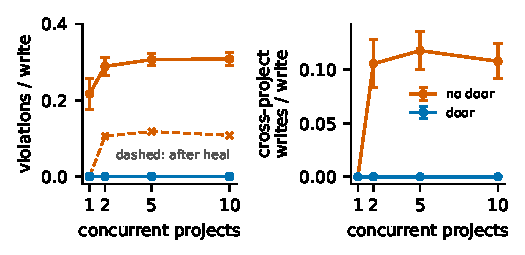
\includegraphics[width=\linewidth]{figs/fig_consistency.pdf}
\caption{RQ1. Left: violations per write, before (solid) and after (dashed) the audit heals. Right: writes landing in another project.}\label{fig:consistency}
\end{figure}

\paragraph*{Cost of the door} The door is 10--19$\times$ slower per write than a raw file write, and its median per-write latency grows 1.5$\times$, 3.3$\times$ and 6.4$\times$ from 1 to 2, 5 and 10 concurrent projects (Fig.~\ref{fig:latency}), because every write opens its own database connection under contention. In absolute terms this remains small relative to an agent step, which takes seconds to minutes, but it is the first scaling bottleneck we observed.

\begin{figure}[t]\centering
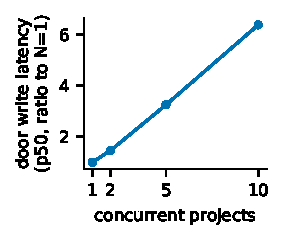
\includegraphics[width=0.55\linewidth]{figs/fig_latency.pdf}
\caption{RQ1. Median door write latency relative to one project.}\label{fig:latency}
\end{figure}

\subsection{RQ2: real LLM agents, before and after}
RQ2 is our main evidence. Table~\ref{tab:rq2} shows the same 54-task experiment (1, 2, 5 and 10 concurrent projects, three repetitions) before and after the changes of Section~\ref{sec:p2}, side by side. Fig.~\ref{fig:rq2p2} plots the two placement measures.

\paragraph*{Before} Task success, measured by running each produced test ourselves, was 100\%, 100\%, 93\% and 97\% (52/54). Agents often wrote \emph{outside the creation door}. Only 67\%, 50\%, 40\% and 17\% of tasks placed their artefacts in their own project's code folder; the rest wrote to a top-level folder of the root, the agent's starting directory. The audit flagged every such stray top-level path (flag ratio 1.0 in every run that had one), but it does not move them automatically. Two further failures appeared at scale. In one repetition at $N=10$, five task names were reused, and four pairs of projects overwrote each other's files in the shared stray folder. In another, an agent wrote one module into another project's folder, and two agents followed the absolute repository path in the system's instructions and wrote into the main workspace instead of their throw-away root.

\paragraph*{Watch stage} With P2a in place and the hook only logging (28 tasks), the hook was invoked on 58 tool calls in the traced run and would have redirected or blocked none of them. All artefacts were in their own code slot. No legitimate write needed routing through the door, so the hook was switched on unchanged.

\paragraph*{After} With the hook enforcing, every task at every $N$ placed its artefacts in its own code slot (1.00), success was 54/54, and no file was written outside a project, into another project, or into the main workspace. The hook allowed every call in this workload and blocked none: starting agents in their own folder (P2a) is what fixed placement for well-behaved agents. Cost per task changed by a factor of 0.79, 0.90, 0.80 and 0.75 relative to the same $N$ before. Its growth with $N$ (ratio to $N=1$: 1.13, 1.19, 1.06) stayed similar to before (0.99, 1.18, 1.13).

\begin{table}[t]
\caption{RQ2 before and after extending the door to the agents' own tools (real LLM agents, 3 repetitions per $N$, 54 tasks per state).}\label{tab:rq2}
\centering\scriptsize
\setlength{\tabcolsep}{3pt}
\begin{tabular}{@{}rccccccc@{}}
\toprule
& & \multicolumn{2}{c}{success} & \multicolumn{2}{c}{own code slot} & \multicolumn{2}{c}{files outside proj./task}\\
\cmidrule(lr){3-4}\cmidrule(lr){5-6}\cmidrule(l){7-8}
$N$ & tasks & before & after & before & after & before & after\\
\midrule
1 & 3 & 1.00 & 1.00 & .67 & \textbf{1.00} & 1.0 & \textbf{0}\\
2 & 6 & 1.00 & 1.00 & .50 & \textbf{1.00} & 1.5 & \textbf{0}\\
5 & 15 & .93 & 1.00 & .40 & \textbf{1.00} & 1.2 & \textbf{0}\\
10 & 30 & .97 & 1.00 & .17 & \textbf{1.00} & 1.7 & \textbf{0}\\
\midrule
\multicolumn{8}{@{}l}{Across all $N$: cross-project modules 1 $\to$ 0; writes into the main workspace 2 $\to$ 0.}\\
\bottomrule
\end{tabular}
\end{table}

\begin{figure}[t]\centering
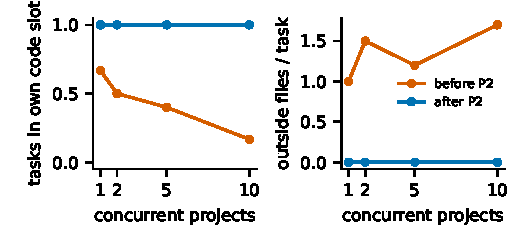
\includegraphics[width=\linewidth]{figs/fig_rq2_p2.pdf}
\caption{RQ2 before (red) and after (blue). Left: share of tasks with all artefacts in the own code slot. Right: files written outside any project per task.}\label{fig:rq2p2}
\end{figure}

\paragraph*{Adversarial variant} Well-behaved agents never tested the hook's blocking, so we asked agents to break the rule (Table~\ref{tab:adv}). With the hook off, all five agents wrote their module directly into the shared library and into another project's code folder. Five modules landed in other projects. The audit flagged none of the shared-library writes, because a file in the shared library is legal at rest. With the hook on, every raw attempt was refused: 9 shell writes into shared code and 5 into another project. No module landed in another project. The agents read the refusal message and promoted their module through the door instead (5/5, confirmed in their transcripts). Promotion leaves a pointer in the project and registers the file, so the shared library changed only through the audited route. One agent's own test failed in this run (4/5).

\begin{table}[t]
\caption{Adversarial variant ($N=5$): each agent is asked to copy its module into the shared library and into another project.}\label{tab:adv}
\centering\scriptsize
\begin{tabular}{@{}lcc@{}}
\toprule
& hook off & hook on\\
\midrule
raw writes into shared code & 5/5 agents & 0 (9 blocked)\\
modules landed in another project & 5 & \textbf{0} (5 blocked)\\
shared modules via the door & 0/5 & \textbf{5/5}\\
audit flags on shared writes & 0 & n/a (door)\\
task tests passing & 5/5 & 4/5\\
\bottomrule
\end{tabular}
\end{table}

\paragraph*{What the adversarial run taught us about the hook} Two weaknesses surfaced, and both were fixed without new rules. In the first hook-on run some agents set the actor variable themselves. They set it to their own project, so no harm resulted, but it showed that the door could have been called under another project's name. The hook now refuses a door call made under a foreign actor, and a door call no longer excuses another raw write chained in the same command. A later owner test exposed two false positives in the hook's shell parser: a \texttt{>} inside a quoted \texttt{sed} expression, and code fed to Python through a here-document, were read as write targets. The parser is now quote- and here-document-aware. All four cases are regression checks. The final adversarial numbers in Table~\ref{tab:adv} come from a re-run with the fixed hook. The first run gave the same blocking result (15 blocked, 0 cross-project modules).

\subsection{RQ3: the owner's own tests, before and after}
Table~\ref{tab:rq3} summarises the owner's four tests. The lifecycle test creates four projects of different shapes through the door, monitors them and deletes them. It was all green in 3/3 runs both before and after the changes. Each creation had zero placement errors and zero violations. The deploy-shaped project reused the shared deploy capability through a pointer, with no second deploy script. Deletion returned every registry count to its exact baseline. The adversarial test injects every violation type and requires the system to correct it on disk and in the database. It passed 32/32 checks in 3/3 runs, before and after. Before the changes it also \emph{failed} once, correctly: it reported the two files that agents had written into the main workspace as cross-project duplicates and refused to declare a clean baseline.

The two LLM-driven tests revealed two defects, which we fixed in the isolated copy.
\begin{itemize}
\item \textbf{Missing role resources.} The most recently added role (\newrole{}) had no resources-and-dependencies section in the role catalogue, so the multi-agent ``Revealer'' build stopped at its own pre-flight gate. We added the catalogue entry, with its dependencies taken from the role's own definition. After the fix, the pre-flight passed and the build ran. The CTO agent then stopped truthfully, before writing any application code: the isolated copy has no credentials (by design), and its rules forbid reporting numbers without a credentialed source. The scorecard therefore moved from ``blocked at pre-flight'' to 5/10 rows (team derivation, planning, CTO present, truthfulness, completed in time). The five build rows cannot pass without credentials. The hook blocked nothing in this run.
\item \textbf{Leftover registry rows.} In the prompt journey (three projects created from prompts), deletion left one or two registry rows behind in 3/3 projects: the files of the project's conversation scopes. The door's delete now removes those scope folders and their rows. After the fix, 2/3 deletions were exactly clean. The third showed one extra row, which is not the project's: the system's own audit log, registered for the first time on the freshly restored database while that project was running. No row owned by any deleted project remained.
\end{itemize}
The journey's other findings did not change: the derived team covered the required capabilities in 1/3 projects, and 2/3 produced output. Both depend on how teams are derived from the prompt, which we did not change. After this test we also found agent processes of already-deleted projects still running. We stopped them and record this as a proposal.

\begin{table}[t]
\caption{RQ3: the owner's own tests, before and after the changes.}\label{tab:rq3}
\centering\scriptsize
\setlength{\tabcolsep}{3pt}
\begin{tabular}{@{}lll@{}}
\toprule
test & before & after\\
\midrule
lifecycle (4 shapes, 3 runs) & all green 3/3 & all green 3/3\\
adversarial (32 checks, 3 runs) & 32/32 $\times$3 & 32/32 $\times$3\\
Revealer pre-flight & blocked (\newrole{} res.) & \textbf{passes}\\
Revealer scorecard & not run & 5/10 (no creds)\\
prompt journey: clean delete & 0/3 (1--2 rows left) & \textbf{2/3} (+1 system row)\\
prompt journey: team coverage & 1/3 & 1/3\\
regression suite & 18/18 & \textbf{32/32}, 0 regressions\\
\bottomrule
\end{tabular}
\end{table}

\subsection{RQ4: queue, callbacks and live sync}
Fig.~\ref{fig:anchor} shows where end-to-end time goes for a request through the \hub{} with zero processing time. Waiting in the queue for the next pull is 97--99\% of the time; submission, publication and callback together are 1--3\%. Four concurrent clients give 2.1$\times$ the throughput of one. With 20\% of callbacks failing, the \hub's own retry sweep delivered 199/200 within the run and the last one at the next sweep (an at-least-once delivery, seen as a duplicate in the following run), so eventual callback success was 100\% in all three repetitions, at the price of retry waits dominating (66--76\% of time). For live sync, a pushed update was visible to a delta reader in under 0.1\% of the poller's push interval; after a restart the mirror and all 20 sequenced messages were present, and a delta request from sequence 15 returned exactly 16--20.

\begin{figure}[t]\centering
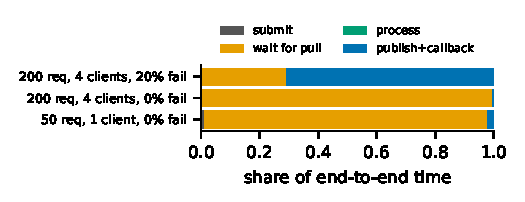
\includegraphics[width=\linewidth]{figs/fig_anchor.pdf}
\caption{RQ4. Share of end-to-end request time per stage (3 repetitions).}\label{fig:anchor}
\end{figure}
